% \documentclass[aip,jcp,preprint,unsortedaddress,a4paper,onecolum]{revtex4-1}
\documentclass[aip,jcp,a4paper,reprint,onecolumn]{revtex4-1}
% \documentclass[aps,pre,twocolumn]{revtex4-1}
% \documentclass[aps,jcp,groupedaddress,twocolumn,unsortedaddress]{revtex4}

\usepackage[fleqn]{amsmath}
\usepackage{amssymb}
\usepackage[dvips]{graphicx}
\usepackage{color}
\usepackage{tabularx}
\usepackage{algorithm}
\usepackage{algorithmic}

\makeatletter
\makeatother

\newcommand{\recheck}[1]{{\color{red} #1}}
\newcommand{\redc}[1]{{\color{red} #1}}
\newcommand{\bluec}[1]{{\color{blue} #1}}
\newcommand{\vect}[1]{\textbf{\textit{#1}}}
\newcommand{\dd}{\textsf{d}}

\newcommand{\mh}{\mathcal H}
\newcommand{\ml}{\mathcal L}
\newcommand{\mt}{\mathcal T}
\newcommand{\fwg}{{\mathcal A}}
\newcommand{\bwg}{{\mathcal B}}
\newcommand{\EX}{{\textrm{EX}}}
\newcommand{\CG}{{\textrm{CG}}}
\newcommand{\HY}{{\Delta}}
\newcommand{\bsigma}{\boldsymbol\sigma}


\begin{document}

\title{Linear response theory for core set identification}
\author{Han Wang}
% \affiliation{Institute for Mathematics, Freie Universit\"at Berlin, Germany}
\author{Christof Sch\"utte}
\affiliation{Institute for Mathematics, Freie Universit\"at Berlin, Germany}
% \affiliation{Institute for Mathematics, Freie Universit\"at Berlin, Germany}

\date{\today}

\begin{abstract}
  % In this draft, we are trying to study the core set based Markov
  % State Model (MSM) under non-equilirbium conditions.
\end{abstract}

\maketitle

\section{Perturbation from equilibrium state}
\subsection{The linear response theory}
In this sub-section, we give a brief description of the linear response
theory, for details see Ref.~\cite{tuckeman2010statistical} for
example. Here we assume the system is governed by the
perturbed Langevin equation:
\begin{align}\label{eqn:langevin-1}
  \dot{\vect q} & = \frac{\partial\mh}{\partial \vect p}
  + \vect C(\vect q,\vect p) F_e(t)\\\label{eqn:langevin-2}
  \dot{\vect p} & =- \frac{\partial\mh}{\partial \vect q}
  + \vect D(\vect q,\vect p) F_e(t)
  - \gamma\vect p
  + \sigma\dot{\vect W}
\end{align}
Where $\vect C$ and $\vect D$ are perturbations to the system, and
$F_e(t)$ is the strength of the perturbation as a function of time.
The phase space incompressibility condition is assumed:
\begin{align}
  \nabla_{\vect q}\cdot\vect C + \nabla_{\vect p}\cdot\vect D = 0
\end{align}
Then the phase space distribution $f(\vect x, t)$ ($\vect x = \{\vect
q, \vect p\}$) is subject to the Kolmogorov forward equation:
\begin{align}
  \frac{\partial}{\partial t} f(\vect x, t) - \fwg f(\vect x, t) = 0
\end{align}
where $\fwg$ is the forward infiniesimal generator given by
\begin{align}
  \fwg =
  \frac{\sigma^2}2\Delta_{\vect p}
  - \Big(
  \frac{\partial \mh}{\partial\vect p} + \vect C F_e(t)
  \Big)\cdot\nabla_{\vect q}
  - \Big(
  -\frac{\partial \mh}{\partial\vect q} +
  \vect D F_e(t) - \gamma\vect p
  \Big)\cdot\nabla_{\vect p}
  + 3N\gamma
\end{align}
The equilibrium and unperturbed system
is governed by
the standard Langevin equation, i.e. with
vanishing input perturbation $F_e(t) = 0$ in
Eqn.~\eqref{eqn:langevin-1} and \eqref{eqn:langevin-2}.
We assume that the perturbation to the
system is so small that both the phase space distribution and the
infiniesimal generator can be viewed as perturbation from the equilibrium
distribution (invariant measure) and the unperturbed operator
($\vect C = \vect D = 0$),
respectively. We have
\begin{align}
  f(\vect x, t) &= f_0(\vect x) + \Delta  f(\vect x, t)
\end{align}
and 
\begin{align}
  \fwg = \fwg_0 + \Delta\fwg(t)
\end{align}
Where the invariant measure satisfies $\fwg_0f_0(\vect x) = 0$,
which is nothing but the Boltzmann distribution
\begin{align}
  f_0(\vect x) \propto e^{-\beta\mh(\vect x)}
\end{align}
The Kolmogorov forward equation for the perturbation is therefore
\begin{align}
  \frac{\partial}{\partial t}
  [f_0(\vect x) + \Delta  f(\vect x, t)]
  -
  [\,\fwg_0 + \Delta\fwg(t)\,]
  [\,f_0(\vect x) + \Delta  f(\vect x, t)\,] = 0
\end{align}
The basic assumption for the ``linear response'' is that the high order
term $\Delta\fwg(t)  \Delta  f(\vect x, t)$ 
can be neglected. Noticing $\fwg_0 f_0(\vect x) = 0$, we have the
Kolmogorov forward equation
for the leading order of the perturbation:
\begin{align}
  \bigg[
  \frac{\partial}{\partial t}
  - \fwg_0
  \bigg]
  \Delta  f(\vect x, t)
  =
  \Delta\fwg(t) f_0(\vect x)
\end{align}
The operator on l.h.s. is the same as the unperturbed equation.
Formally solving this equation with initial condition
$\Delta f(\vect x, 0) = 0$ gives
\begin{align}
  \Delta  f(\vect x, t) =
  \int_0^t \dd s \:
  e^{(t-s)\fwg_0}
  \Delta\fwg(s)f_0(\vect x)
\end{align}
By defining the \emph{dissipative flux},
\begin{align}
  j(\vect x) =
  -\vect C\cdot\nabla_{\vect q}\mh 
  -\vect D\cdot\nabla_{\vect p}\mh
\end{align}
it has been shown that %~\cite{tuckeman2010statistical}
\begin{align}
  \Delta\fwg(s)f_0(\vect x) =
  -\beta f_0(\vect x)\, j(\vect x) F_e(s)
\end{align}
For any observation:
\begin{align}\nonumber
  \mathcal O(t)
  &=
  \int\dd \vect x \:O(\vect x)f(\vect x, t)  \\\nonumber
  &=
  \int\dd \vect x\, O(\vect x)\,
  [f_0(\vect x) + \Delta f(\vect x, t)] \\\nonumber
  &=
  \langle O\rangle_0
  -
  \beta
  \int \dd \vect x\:
  O(\vect x)
  \int_0^t\dd s\,
  e^{(t-s)\fwg_0}
  f_0(\vect x)\, j(\vect x)F_e(s)  \\\nonumber
  &=
  \langle O\rangle_0
  -
  \beta
  \int_0^t\dd s\,
  F_e(s)
  \int \dd \vect x\,
  O(\vect x)\,
  e^{(t-s)\fwg_0}
  f_0(\vect x) j(\vect x)  \\\nonumber
  &=
  \langle O\rangle_0
  -
  \beta
  \int_0^t\dd s\,
  F_e(s)
  \int \dd \vect x\,
  f_0(\vect x) j(\vect x)\,
  e^{(t-s)\bwg_0}
  O(\vect x)\\ \label{eqn:eqi-pert-1}
  &=
  \langle O\rangle_0
  -
  \beta
  \int_0^t\dd s\,
  F_e(t-s)
  \int \dd \vect x\,
  f_0(\vect x) j(\vect x)\,
  e^{s\bwg_0}
  O(\vect x)
\end{align}
Where $\bwg_0$ is the infiniesimal generator of the \emph{unperturbed} 
Kolmogorov backward equation, which is the adjoint operator of $\fwg_0$.
We have
\begin{align}
  e^{s\bwg_0} O(\vect x) = \mathbb E_{\vect x} [O(\vect X_s)]
\end{align}
where $\vect X_t$ is the trajectory of the unperturbed Langevin equation
starting at $\vect x$.
Therefore, we have
% Notice that $e^{i\ml_0(t-s)}O(\vect x) = O(\phi_{t-s}(\vect x))$,
% where $\phi_t(\vect x)$ is the flow mapping of the \emph{unperturbed}
% Hamiltonian system. We have
\begin{align}
  \mathcal O(t)
  =
  \langle O\rangle_0
  -
  \beta
  \int_0^t\dd s\,
  F_e(t-s)
  \int \dd \vect x\,
  f_0(\vect x)
  j(\vect x)\,
  \mathbb E_{\vect x} [O(\vect X_s)]
\end{align}
or equivalently:
\begin{align}\label{eqn:lr}
  \mathcal O(t)
  =
  \langle O\rangle_0
  -
  \beta
  \int_0^t\dd s\,
  F_e(t-s)
  \langle
  j(0)\,
  \mathbb E_{\vect x} [O(\vect X_s)]
  \rangle_0
\end{align}
where $  \langle
  j(0)\,
  \mathbb E_{\vect x} [O(\vect X_s)]
  \rangle_0$ is the \emph{equilibrium time
  correlation} between the observation $O$ at time $s$ and the
dissipative flux $j$ at time 0.


\subsection{The core set as an observation of the system}

The core set plays a very important role in the MSM theory. One way to
identify core set is to consider the ``stability'' of the invariant
measure $f_0$ under a propagator $\mt_\alpha$
of time step $\alpha$, which is associated with a
stochastic process denoted by $\vect Y_\alpha$:
\begin{align}
  C_\alpha = \big\{
  \vect x \,\vert\, \mt_\alpha f_0(\vect x) > f_0(\vect x)
  \big\}
\end{align}
Generally, it is impossible and not necessary to consider the core set
in the $3N$ dimensional configuration space. For example, a
macromolecule solving in water, the DOFs of water is not of interest
at all. Therefore, we consider some phase space compressing function
$\vect y = \vect y(\vect x)$, with $\vect y \in \Omega \subset \mathbb
R^M,\ M\ll 3N$. We call $\Omega$ the observation space.  The projected
invariant measure on the observation space is therefore
\begin{align}
  \mathcal P f_0 (\vect y)
  =
  \int
  \dd \vect x\,
  f_0(\vect x) \,
  \delta (\vect y - \vect y(\vect x)) 
\end{align}
The core set on the observation space is
\begin{align}
  \widetilde
  C_\alpha = \big\{
  \vect y \,\vert\,
  \mathcal P\mt_\alpha f_0(\vect y) > \mathcal P f_0(\vect y)
  \big\}
\end{align}
% with $\widetilde \mt_\alpha$ defined by
% $\widetilde\mt_\alpha = \mathcal P\circ\mt_\alpha$, namely
% \begin{align}
%   \widetilde\mt_\alpha\, p_0(\vect y)
%   =
%   \mathcal P\circ\mt_\alpha f_0 (\vect y)
%   =
%   \int
%   \dd \vect x\,
%   [\mt_\alpha f_0](\vect x) \,
%   \delta (\vect y - \vect y(\vect x)) 
% \end{align}
For convenience, we define $\Delta \mt_\alpha =
\mt_\alpha - \mathcal I$, where $\mathcal I$ is the
identity. If $[\mathcal P\circ\Delta \mt_\alpha f_0](\vect y) > 0$, then
$\vect y$ is in the core set $\widetilde C_\alpha $.
\begin{align}\nonumber
  [\mathcal P\circ\Delta \mt_\alpha f_0](\vect y)
  &=
  \int
  \dd \vect x\,
  \Delta \mt_\alpha f_0(\vect x) \,
  \delta (\vect y - \vect y(\vect x))  \\\nonumber
  &=
  \lim_{\sigma \rightarrow 0}
  \int
  \dd \vect x\,
  \Delta \mt_\alpha f_0(\vect x) \,
  K_{\sigma} (\vect y - \vect y(\vect x))  \\\nonumber
  &=
  \lim_{\sigma \rightarrow 0}
  \int
  \dd \vect x\,
  \Delta \mt_\alpha f_0(\vect x) \,
  K_{\sigma, \vect y} (\vect x)  \\\nonumber
  &=
  \lim_{\sigma \rightarrow 0}
  \int
  \dd \vect x\,
  f_0(\vect x) \,
  [\Delta \mt_\alpha]^\dagger K_{\sigma, \vect y} (\vect x)\\
  &=
  \lim_{\sigma \rightarrow 0}\,
  \langle
  [\Delta \mt_\alpha]^\dagger K_{\sigma, \vect y}
  \rangle_0
\end{align}
where $[\Delta \mt_\alpha]^\dagger$ is the adjoint operator of $\Delta
\mt_\alpha$. The delta
function is replaced by the limit of a mollifier $K_\sigma(\vect y)$,
which is infinitely smooth, compact supported of size $\sigma$,
bounded and $\int
K_\sigma(\vect y)\dd \vect y = 1$.  The physical meaning is that we
can consider the expectation value of the stability of the mollifier
$K_{\sigma, \vect y}$ instead of the stability of the invariant measure.
This provides the convenience of using the linear response theory showed
in the previous section. By Eqn.~\eqref{eqn:lr},
\begin{align}\nonumber
  [\mathcal P\circ\Delta \mt_\alpha f_t](\vect y)
  &=
  \lim_{\sigma \rightarrow 0}\,
  \langle
  [\Delta \mt_\alpha]^\dagger K_{\sigma, \vect y}
  \rangle_t \\\nonumber
  &=
  \lim_{\sigma \rightarrow 0}\,
  \Big\{
  \langle
  [\Delta \mt_\alpha]^\dagger K_{\sigma, \vect y}
  \rangle_0  -
  \beta
  \int_0^t\dd s\,
  F_e(t-s)
  \langle
  j(0)\,
  \mathbb E_{\vect x}\{
  [\Delta \mt_\alpha]^\dagger K_{\sigma, \vect y}(\vect X_s)\,
  \}
  \rangle_0
  \Big\} \\ \label{eqn:main}
  &=
  \lim_{\sigma \rightarrow 0}\,
  \Big\{
  \langle
  [\Delta \mt_\alpha]^\dagger K_{\sigma, \vect y}
  \rangle_0  -
  \beta
  \int_0^t\dd s\,
  F_e(t-s)
  \Big\langle
  j(0)\,
  \mathbb E_{\vect x}
  \big[
  \mathbb E_{\vect X_s}
  (K_{\sigma, \vect y}(\vect Y_\alpha))
  -
  K_{\sigma, \vect y}(\vect X_s)
  \big]
  \Big\rangle_0
  \Big\}
\end{align}
with initial conditions:
\begin{align}
  \vect X_0 = \vect x; \quad \vect Y_0 = \vect X_s.
\end{align}
Therefore, the core set at time $t$ is defined by
\begin{align}
  \widetilde C_\alpha^t =
  \Big\{
  \vect y
  \,\Big\vert\,
  [\mathcal P\circ\Delta \mt_\alpha f_t](\vect y) > 0
  \Big\}
\end{align}


\begin{figure}
  \centering
  \includegraphics[width=0.35\textwidth]{figs/fig-pot.eps}
  \caption{The potential with and without perturbation.}
  \label{fig:tmp1}
\end{figure}


\subsection{Numerical test}

We test the idea by a one-dimensional model system: one particle in a
double-well potential. For convenience, we let the mass of the
particle to be 1 \textsf{amu}. The Hamiltonian of the system is given
by:
\begin{align}
  \mh (\vect p, \vect q) = \frac 12 \vect p^2 + U(\vect q) 
\end{align}
with
\begin{align}
  U(\vect q) = \frac12 k (\vect q^2 - a^2)^2
\end{align}
Here $k = 8$ $\textsf{kJ} / (\textsf{mol nm}^4)$, and $ a = 1 \textsf{nm}$.
Notice at room temperature $300 \textsf{K}$, $k_BT = 2.48$ \textsf{kJ/mol}.
See the red line in Fig.~\ref{fig:tmp1}.
%$\textsf{kJ} / (\textsf{mol nm}^4)}$
The perturbation is given by
\begin{align}
  \vect C(\vect p, \vect q) = 0; \qquad
  \vect D(\vect p, \vect q) = -\nabla_{\vect q} V(\vect q) = 1
\end{align}
Here $V(\vect q) = -\vect q$, which effectively tilt the original
potential $U(\vect q)$. The strength of the perturbation $F_e(t)$ is given
by the following function:
\begin{align}
  F_e(t) = 
  \begin{cases}
    F_e^{\textrm{max}}\times (t / t_c) & t < t_c \\
    F_e^{\textrm{max}} & t \geq t_c
  \end{cases}
\end{align}
$t_c = 100$ \textsf{ps} so that the perturbation increases slow
enough: the typical decaying time scale of the correlation function
in~\eqref{eqn:main} is roughly 3 \textsf{ps}.  We choose $\mt_\alpha$
to be the propagator of the Langevin dynamics at temperature $150$
\textsf{K} with $\alpha = 1$ \textsf{ps}.  Since the dynamics is in
1-d, the projection is identity.  We consider the stability of the
distribution $f_t$ at time $t$: $-\Delta\mt_\alpha f_t$. The smaller
this value, the more stable the core sets are.

See Fig. \ref{fig:tmp2} and \ref{fig:tmp3} for numerical result.  Both
the direct non-equilibrium simulation and the linear response
approximation are presented. Time slices $t = 0$, 30, 60 and 100
\textsf{ps} are shown.  When the perturbation is small,
i.e. $F_e^{\textrm{max}} = 2$, the direct non-equilibrium simulation
and the linear response results consistent very well. As the
perturbation grows stronger, the left well becomes less stable, while
the right well becomes more stable.  When the perturbation is big,
i.e. $F_e^{\textrm{max}} = 6$, the linear response results are no
longer precise. When $t\geq 60$ \textsf{ps}, the left well basically
disappears, however, the linear response calculation present a well
that is nearly as stable as the right well.

\begin{figure}
  \centering
  \includegraphics[width=0.95\textwidth]
  {figs/warm100.str2.0.nst1e09.smallgrid/fig-2d.eps}
  \caption{The stability of distribution $f_t$ under perturbation of
    $F_e^{\textrm{max}} = 2$.
    Upper row: the direct non-equilibrium simulation. Lower row: the
    results of linear response formula~\eqref{eqn:main}.
  }
  \label{fig:tmp2}
\end{figure}

\begin{figure}
  \centering
  \includegraphics[width=0.95\textwidth]
  {figs/warm100.str6.0.nst1e09.smallgrid/fig-2d.eps}
  \caption{The stability of distribution $f_t$ under perturbation of
    $F_e^{\textrm{max}} = 6$.  Upper row: the direct non-equilibrium
    simulation. Lower row: the results of linear response
    formula~\eqref{eqn:main}.  }
  \label{fig:tmp3}
\end{figure}


\section{Non-equilibrium linear response}

\subsection{Path integral}
The path integral is very useful to develop the non-equilibrium version of
linear response theory. 
Comparing with the idea of ensemble, which is a collection of state points
in the configuration space, the path integral consider the ``ensemble'' of
trajectories.
(In the following, the develop of formula are formal. The strict mathematical
theory is still unclear for me.)
First, we take the standard 1-dimensional Wiener process for example.
Consider the time interval $[0,T]$, the probability density of one trajectory
is given by
\begin{align}
  p[W_t] = \frac 1Z e^{-I[W_t]}
\end{align}
where $I$ is the action functional of Wiener process given by
\begin{align}
  I[W_t] = \int_0^T\frac12 \dot{W}_t^2\dd t
\end{align}
the partition function $Z$ is
\begin{align}
  Z = \int  e^{-I[W_t]} \prod_{0\leq t\leq T}\dd W_t
\end{align}
Consider the following two stochastic processes:
\begin{align}\label{eqn:st-orig}
  \dd \vect X_t &= \vect b(\vect X_t, t) \dd t + \bsigma(\vect X_t, t)\,\dd\vect W_t \\\label{eqn:st-pert}
  \dd \vect Y_t &= \vect b(\vect Y_t, t) \dd t + \vect c(\vect Y_t, t) \dd t + \bsigma(\vect Y_t, t)\,\dd\vect W_t
\end{align}
Where $\vect W_t$ is the standard Wiener process. Obviously
\eqref{eqn:st-pert} is the perturbed version of
\eqref{eqn:st-orig}. It has been shown that, starting from the same
measure saying $\mu$ (which is not necessarily equilibrium or
stationary), the ratio of trajectory probability density between the perturbed
and unperturbed process is~\cite{li2010lecture} (\recheck{I think here
  the incompressibility of phase space should be assumed. Otherwise the
  ratio should be more complicated.})
\begin{align}\label{eqn:girsanov}
  \frac{\dd\mathcal P_{\vect Y}}{\dd\mathcal P_{\vect X}}
  =
  \exp
  \Big\{
  -\frac12 \int_0^T\vert\bsigma^{-1}\cdot\vect c(\vect X_t,t)\vert^2\,\dd t
  +\int_0^T[\dot{\vect X}_t - \vect b(\vect X_t,t)]^T
  \cdot\bsigma^{-T}\cdot\bsigma^{-1}\cdot\vect c(\vect X_t,t)\,\dd t 
  \Big\}
\end{align}
where $\mathcal P_{\vect Y}$ and $\mathcal P_{\vect Y}$ are measures
of the trajectories generated by \eqref{eqn:st-pert} and
\eqref{eqn:st-orig}, respectively.  This result (Girsanov formula?) is
(formally) precise without any approximation.


\subsection{Non-equilibrium perturbation with linear approximation}

To be more general, we study the two perturbed Langevin dynamics
(i.e. Eqn.~\eqref{eqn:langevin-1} and \eqref{eqn:langevin-2}) with
different perturbations that are given by $F_e^1(t)$ and $F_e^2(t)$,
respectively. We consider the difference between the observations of
these dynamics:
\begin{align}\label{eqn:noneq-pert-1}
  \langle Q(t)\rangle_{\mu}^{2}  -\langle Q(t)\rangle_{\mu}^{1}
  &=
  \int Q(\vect X_t) \,\dd\mathcal P^2[\vect X_t]
  -\int Q(\vect X_t) \,\dd\mathcal P^1[\vect X_t]
  =
  \int Q(\vect X_t)
  \Big\{
  \frac{\dd\mathcal P^2[\vect X_t]}{\dd\mathcal P^1[\vect X_t]}
  -1
  \Big\}
  \,\dd\mathcal P^1[\vect X_t]
\end{align}
\recheck{Here we further assume that $\vect C(\vect q, \vect p) = 0$.
  (otherwise the Girsanov formula~\eqref{eqn:girsanov} may be unstable...
  By letting the $\epsilon$ in the following formula to 0, if
  $\vect C\neq 0$, the limit may not be exist. This
  is intuitionally not likely... I do not know why.)}
By writing Eqn.~\eqref{eqn:langevin-1} and \eqref{eqn:langevin-2} as
\begin{align}
  \frac{\dd }{\dd t}
  \left[
    \begin{array}{l}
      \vect q\\
      \vect p
    \end{array}
  \right]
  =
  \left[
    \begin{array}{l}
      \nabla_{\vect p}\mh\\
      -\nabla_{\vect q}\mh - \gamma\vect p + F_e\vect D
    \end{array}
  \right]
  \dd t
  +
  \left[
    \begin{array}{cc}
      \epsilon \vect I & 0\\
      0 & \sigma\vect I
    \end{array}
  \right]
  \cdot
  \left[
    \begin{array}{l}
      \dd\vect W_t\\
      \dd\vect W_t
    \end{array}
  \right]
\end{align}
Using Girsanov's formula, to the leading order of $\Delta F_e = F_e^2 - F_e^1$,
we have
\begin{align}\nonumber
  \frac{\dd\mathcal P^2[\vect X_t]}{\dd\mathcal P^1[\vect X_t]}
  -1
  &=
  \exp
  \Big\{
  \frac 1 {\sigma^2}
  \int_0^t
  [\dot{\vect p}_s +
  \gamma\vect p_s +
  \nabla_{\vect q}\mh(\vect q_s,\vect p_s)
  - F_e^1(s) \vect D(\vect q_s,\vect p_s)
  ]\cdot
  \vect D(\vect q_s,\vect p_s)
  \Delta F_e(s)\,
  \dd s
  + \mathcal O(\Delta F_e^2)
  \Big\} - 1 \\\label{eqn:girsanov-langevin-1}
  &\approx
  \frac 1 {\sigma^2}
  \int_0^t
  [\dot{\vect p}_s +
  \gamma\vect p_s +
  \nabla_{\vect q}\mh(\vect q_s,\vect p_s)
  - F_e^1(s) \vect D(\vect q_s,\vect p_s)
  ]\cdot
  \vect D(\vect q_s,\vect p_s)
  \Delta F_e(s)\,
  \dd s  
\end{align}
This is where the \emph{linear approximation} applies.
By using the relation $\beta = 2\gamma / \sigma^2$ and split the
Eqn.~\eqref{eqn:girsanov-langevin-1} into time symmetric and
antisymmetric parts~\cite{baiesi2010nonequilibrium2}, we have:
\begin{align}\nonumber
  \frac{\dd\mathcal P^2[\vect X_t]}{\dd\mathcal P^1[\vect X_t]}
  -1
  \approx& \:
  \frac\beta 2
  \int_0^t
  \Delta F_e(s)\,
  \vect p_s\cdot \vect D(\vect q_s,\vect p_s)\,
  \dd s\\  \label{eqn:girsanov-langevin-2}
  &\,-
  \frac 1{\sigma^2}
  \int_0^t
  \Delta F_e(s)\,
  \vect F^1(\vect q_s,\vect p_s)\cdot \vect D(\vect q_s,\vect p_s)\,
  \dd s  
  +
  \frac 1{\sigma^2}
  \int_0^t
  \Delta F_e(s) \vect D(\vect q_s,\vect p_s)\cdot \dd \vect p_s,
\end{align}
where $\vect F^1(\vect q_s,\vect p_s) = -\nabla_{\vect q}\mh(\vect
q_s,\vect p_s) + F_e^1(t) \vect D(\vect q_s,\vect p_s)$.  The first
line of the r.h.s. of Eqn.~\eqref{eqn:girsanov-langevin-2} is the time
integrated excess entropy flux, which is time-antisymmetric, while the
second line is the excess dynamic activity that is time-symmetric.
Inserting Eqn.~\eqref{eqn:girsanov-langevin-2} into
\eqref{eqn:noneq-pert-1}, we have
\begin{align}\nonumber
  \langle O(t)\rangle_{\mu}^{2}  -\langle O(t)\rangle_{\mu}^{1}
  =&\,
  \frac\beta 2
  \int_0^t\dd s\,
  \Delta F_e(s)\,
  \big\langle
  \vect p_s\cdot\vect D(\vect X_s)\,O(\vect X_t)
  \big\rangle_\mu^1 \\  \label{eqn:noneq-pert-2}
  &
  -
  \frac1{\sigma^2}
  \int_0^t\dd s\,
  \Delta F_e(s)\,
  \big\langle
  \vect F^1(\vect X_s)\cdot\vect D(\vect X_s)\,O(\vect X_t)
  \big\rangle_\mu^1
  +
  \frac1{\sigma^2}
  \int_0^t
  \Delta F_e(s)\,
  \big\langle
  \dd \vect p_s\cdot\,
  \vect D(\vect X_s)\,O(\vect X_t)
  \big\rangle_\mu^1  
\end{align}
If $\vect D(\vect x)$ is independent of momentum and is conservative,
saying $\vect D(\vect x) = \vect D(\vect q) = -\nabla_{\vect q}
V(\vect q)$, then the last term of \eqref{eqn:noneq-pert-2} can be
further simplified, because
\begin{align}
  -\dd\, [\nabla_{\vect q}V(\vect q_s)\cdot \vect p_s]
  =
  -\nabla_{\vect q}V(\vect q_s)\cdot\dd \vect p_s
  - \vect p_s\cdot\nabla^2_{\vect q}V(\vect q_s)\cdot\vect p_s\,\dd s,
\end{align}
then \eqref{eqn:noneq-pert-2} changes to
\begin{align}\nonumber
  \langle O(t)\rangle_{\mu}^{2}  -\langle O(t)\rangle_{\mu}^{1}
  =&\,
  -\frac\beta 2
  \int_0^t\dd s\,
  \Delta F_e(s)\,
  \big\langle
  \vect p_s\cdot\nabla_{\vect q} V(\vect X_s)\,O(\vect X_t)
  \big\rangle_\mu^1 \\\nonumber
  & +
  \frac1{\sigma^2}
  \int_0^t\dd s\,
  \Delta F_e(s)\,
  \big\langle
  \vect F^1(\vect X_s)
  \cdot\nabla_{\vect q} V(\vect X_s)
  \,O(\vect X_t)
  \big\rangle_\mu^1 \\\nonumber
  & -
  \frac1{\sigma^2}
  \int_0^t
  \dd s\,
  \Delta F_e(s)\,
  \frac{\dd}{\dd s}
  \big\langle
  \vect p_s\cdot\,
  \nabla_{\vect q} V(\vect X_s)
  \,O(\vect X_t)
  \big\rangle_\mu^1    \\\label{eqn:noneq-pert-3}
  & +
  \frac1{\sigma^2}
  \int_0^t
  \dd s\,
  \Delta F_e(s)\,
  \big\langle
  \vect p_s\vect p_s:
  \nabla^2_{\vect q} V(\vect X_s)
  \,O(\vect X_t)
  \big\rangle_\mu^1      
\end{align}

\subsection{Remarks and possibilities}
\bluec{
\begin{itemize}
\item It can be shown that 
  Eqn.~\eqref{eqn:noneq-pert-3} simply reduces to
  \eqref{eqn:eqi-pert-1}
  in the equilibrium case~\cite{baiesi2010nonequilibrium2}.
\item  Eqn.~\eqref{eqn:noneq-pert-3} shows that the trajectory average of
  $F_e^2$ is calculated from the trajectory average of $F_e^1$. We
  assume: (1) they start from the same initial distribution $\mu$, and
  (2) $F_e^2$ is not very far from $F_e^1$ so that the linear
  approximation is reasonably valid.  The condition (1) can be made
  weaker, for example $F_e^2$ starts from $\mu_2$ and $F_e^1$ starts
  from $\mu_1$, however, $\mu_2$ should be similar to $\mu_1$,
  otherwise the sampling is of poor accuracy.
  (2) means all possible trajectories of perturbation $F_e^2$ should be
  effciently sampled by perturbation $F_e^1$.
\item Eqn.~\eqref{eqn:noneq-pert-3}, may be used in this way:
  assume we want to study the dynamics of $F_e^2$, which is very slow
  and difficult to handle directly.
  We can instead study the dynamics of $F_e^1$, which is
  similar to $F_e^2$, but is much faster, so that it can be handle by MD.
  And then use \eqref{eqn:noneq-pert-3} to calculate the averages of
  the target dynamics $F_e^2$.
  A possible choice of  $F_e^1$ may be  $F_e^1 = \alpha F_e^2,\ \alpha > 1$.
  On the other hand, perturbation $F_e^2$ should be not very far
  from $F_e^1$, that means $F_e^2$ can not arbitrarily accelerate
  $F_e^1$. Fortunately we have the freedom to design $F_e^2$, therefore,
  an error estimate may help, and a path optimization of $F_e^2$
  may be developed.
\item The perturbation $F_e^1$ can be kept a constant so that the
  system reaches a stationary state.
  $F_e^2$ is perturbation from that stationary state.
  The averages in
  \eqref{eqn:noneq-pert-3} can be calculated easier, because
  what we sample is the stationary state, rather the trajectories.
  When the system is far from the stationary state, the
  accuracy is low. 
\item It may also be possible to study multiple reference dynamics,
  and use interpolations to increase the accuracy of the linear
  approximation.
\item Extension to nonlinear response?
\end{itemize}
}

\section*{References}
\bibliography{ref}{}
\bibliographystyle{unsrt}





\end{document}